% ----------------------------------------------------------
\chapter{Visão Geral do Projeto}
% ----------------------------------------------------------



% ----------------------------------------------------------
\section{Contextualização}
% ----------------------------------------------------------

O endividamento de famílias brasileiras atingiu 78,1\% em março de 2024 de acordo com CNC (2024). Isso representa que aproximadamente 8 a cada 10 famílias possuem algum tipo de dívida, seja ela atrasada ou não. É considerada inadimplente a parcela da população que possui dívidas atrasadas, ou seja, deixou de pagar uma dívida no vencimento ou o não cumprimento de um contrato ou clausula de contrato (Sehn et Carlini Junior, 2007).

A parcela inadimplente das famílias brasileiras representou 28,5\% em março de 2024 segundo CNDL (2024). O alto nível de inadimplência retrata não apenas as dificuldades econômicas enfrentadas num pais, mas partindo de um olhar microeconômico  situações comuns como desemprego, despesas inesperadas, falta de planejamento financeiro, compras para terceiros e ausência de educação financeira (SPC,2024).

De acordo com  Serasa (2024), as principais dividas por segmento em fevereiro de 2024 são: Cartão de Crédito com 29,27\%, contas básicas como água e luz são 22,67\%, financeiras com 17,17\% e varejo com 10,99\%. O fato do cartão de crédito ser a principal forma de inadimplência, pode ser interpretado que ele seja entendido como uma extensão de renda mensal das pessoas, no entanto, o que acontece é um empréstimo pré-estabelecido a ser pago posteriormente.

Os impactos sofridos pelo endividamento vão além do financeiro, segundo Serasa (2022) aponta que 83\% dos devedores têm dificuldade para dormir, 78\% dos entrevistados têm surtos de pensamentos negativos devido em relação as inadimplências e 61\% têm crises de ansiedade ao pensar na dívida. Os dados apresentados ressaltam que possuir uma vida financeira saudável contribui não só com saúde mental mas com a satisfação das necessidades fisiológicas do cidadão: moradia e alimentação, isso vai de encontro com Araújo e Souza (2012), cujas ideias, expressam que com um planejamento melhor da vida financeira e menos envolvimento com necessidade de crédito torna a saúde financeira mais fundamentada.  

 Por conta da importância dada à educação financeira, foi criada em 2010 a Estratégia Nacional de Educação Financeira (ENEF), cujo principal objetivo é promover a educação financeira e previdenciária de acordo com MEC(2024). A ENEF é governamental e possui mais de 1300 iniciativas relacionadas a educação financeira (CUNHA, 2022). Diante desse cenário, surge a necessidade de ferramentas práticas que auxiliem os indivíduos a aplicarem os conhecimentos adquiridos em sua rotina financeira. 

Nesse contexto, o desenvolvimento de uma aplicação web dedicada à gestão financeira pode representar um passo significativo. Esta aplicação não apenas facilitaria o dia a dia dos usuários ao oferecer funcionalidades de controle e planejamento financeiro, mas também serviria como uma plataforma interativa de aprendizado contínuo em finanças, alinhando-se assim aos objetivos da ENEF de fomentar a educação financeira de maneira acessível e prática.

Diante dos problemas e oportunidades apresentadas, o principal objetivo deste trabalho é desenvolver uma aplicação web, que auxilie o usuário com a gestão financeira, permitindo e a visualização de suas finanças de forma simples.


% ----------------------------------------------------------
\section{Descrição do projeto do Produto}
% ----------------------------------------------------------


Este projeto visa desenvolver um aplicativo móvel focado na gestão financeira individual, oferecendo aos usuários a capacidade de gerir o próprio orçamento, além de documentar e categorizar receitas e gastos para uma melhor análise e visualização.

O aplicativo Web inclui funcionalidades como a geração de gráficos de despesas segregados por categoria e a exibição do saldo mensal total, facilitando aos usuários uma compreensão mais clara de suas finanças. Esses recursos visam auxiliar na tomada de decisões financeiras mais informadas e baseadas em dados concretos.

Em síntese, a aplicação Web é projetada para proporcionar aos usuários uma gestão financeira mais efetiva. Ao facilitar o registro organizado de receitas e despesas, categorizando-as e apresentando insights valiosos sobre o comportamento de gastos e rendimentos ao longo de diversos intervalos temporais, os usuários ganham um controle aprimorado sobre sua saúde financeira.

% ----------------------------------------------------------
\section{Funcionalidades}
% ----------------------------------------------------------

\begin{itemize}
    \item Usuário gera um cadastro para si mesmo, assim como uma senha;
    \item Usuário cria categorias para entrada ou saida de dinheiro;
    \item Usuário cria orçamentos mensais;
    \item Usuário criar filtros para seus lançamentos
\end{itemize}

% ----------------------------------------------------------
\section{Tecnologias Usadas}
% ----------------------------------------------------------

As escolhas das tecnologias foram baseadas em 3 fatores: relevância no mercado de trabalho, documentação extensiva disponível na internet, curva de aprendizagem. Com a escolha da ferramentas, a arquitetura da aplicação pode ser definida e é mostrada na figura \ref{fig:process_macro}: 



\begin{figure}[htb]
	\caption{\label{fig:process_macro}Processo macro.}
	\begin{center}
		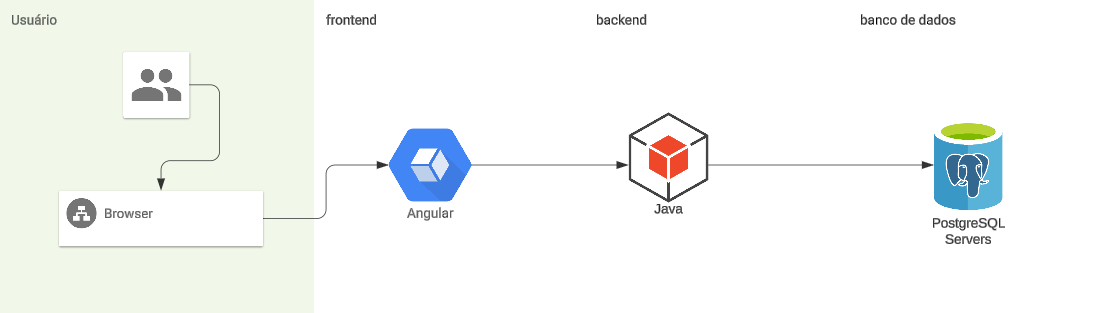
\includegraphics[scale=0.5]{images/processoMacro.png}
	\end{center}
	\fonte{Autor (2024)}
\end{figure}

Como pode ser visto na figura \ref{fig:process_macro} as principais ferramentas são definidas em:

\begin{itemize}
    \item Frontend: Interface de usuário baseada na linguagem Angular;
    \item Backend: API REST programada em Java, com SpringBoot;
    \item Banco de dados: Banco de dados relacional PostgreSQL.
\end{itemize}

\subsection{Java}

 Java é uma linguagem de programação orientada a objetos que é conhecida por sua portabilidade entre plataformas, o que significa que programas escritos em Java podem ser executados em qualquer dispositivo que possua a máquina virtual Java (JVM). Amplamente utilizada para o desenvolvimento de aplicações empresariais, sistemas de gerenciamento de bancos de dados, aplicativos móveis e sistemas embarcados, Java é apreciada por sua robustez, segurança e escalabilidade.

\subsection{SpringBoot}

Spring Boot é um projeto da vasta plataforma Spring que facilita o processo de configuração e publicação de aplicações baseadas em Spring. Esta ferramenta oferece uma maneira rápida e altamente eficaz de desenvolver aplicações stand-alone que podem ser executadas em produção quase que imediatamente. Spring Boot é notável por simplificar o processo de desenvolvimento, oferecendo configurações automáticas e um vasto conjunto de funcionalidades que aceleram o desenvolvimento de aplicações Spring.

\subsection{Angular}

Angular é um framework de desenvolvimento para a construção de aplicações web dinâmicas. Utilizando TypeScript como linguagem principal, Angular oferece aos desenvolvedores uma arquitetura robusta para a construção de interfaces de usuário ricas e interativas, com recursos como data-binding bidirecional, injeção de dependência e um sistema de rotas extensivo. Angular é especialmente benéfico para projetos que necessitam de uma estrutura organizada e escalável para aplicações de página única (SPA).

\subsection{PostgreSQL}

PostgreSQL é um sistema de gerenciamento de banco de dados relacional avançado, conhecido por sua robustez e conformidade com os padrões SQL. É uma solução de código aberto amplamente utilizada em todo o mundo por sua capacidade de lidar com grandes volumes de dados, extensa capacidade de personalização e suporte a uma vasta gama de tipos de dados, incluindo tipos geométricos e de rede. PostgreSQL se destaca pela sua arquitetura sofisticada que suporta transações, subconsultas, triggers, views e procedimentos armazenados, tornando-o uma escolha ideal para aplicações complexas e sistemas que exigem alta integridade de dados. Além disso, é altamente extensível, permitindo aos desenvolvedores adicionar novas funções, tipos de dados e até mesmo escrever código em diferentes linguagens de programação diretamente no banco de dados. Esta flexibilidade faz do PostgreSQL uma opção poderosa tanto para pequenas aplicações quanto para grandes empresas que necessitam de um sistema de banco de dados confiável e escalável.

\subsection{Notion}

Notion é uma aplicação versátil de organização e produtividade que permite aos usuários criar, compartilhar e gerenciar notas, tarefas, bancos de dados e wikis, tudo em um único espaço. A plataforma é altamente flexível, permitindo uma personalização extensa para se adequar a diferentes necessidades de fluxos de trabalho, seja para uso pessoal, acadêmico ou profissional. O Notion se destaca por sua interface de usuário intuitiva e capacidades de colaboração em tempo real. 

\subsection{Lucidchart}

Lucidchart é uma plataforma online de diagramação e visualização de dados que facilita a criação de diagramas complexos usados em diversas áreas, como engenharia de software, design de rede e processos de negócios. Com uma interface drag-and-drop, Lucidchart permite aos usuários colaborar em tempo real, tornando-o uma ferramenta ideal para equipes remotas e projetos que exigem planejamento visual e organização de ideias complexas.


\subsection{Hardware}

O hardware utilizado no desenvolvimento e testes foi um PC desktop com as configurações:

\begin{itemize}
    \item Processador: AMD Ryzen 5 5500;
    \item Placa mãe: MSI B550M PRO-VDH
    \item Memória RAM: 16 GB
    \item Memoria ROM: 1TB SSD
\end{itemize}

\nocite{cnc2024}
\nocite{SPCetCDNL}
\nocite{serasa}
\nocite{serasa2022}
\nocite{Sehn}
\nocite{araujo}
\nocite{MEC}
\nocite{larrisaENEF}